\chapter{Discrete-time Signals in the Frequency Domain}
In physics, electronics, control systems engineering, and statistics, the \textbf{frequency domain} refers to the analysis of mathematical functions or signals with respect to frequency, rather than time. Put simply, a time-domain graph shows how a signal changes over time, whereas a frequency-domain graph shows how much of the signal lies within each given frequency band over a range of frequencies. A frequency-domain representation can also include information on the phase shift that must be applied to each sinusoid in order to be able to recombine the frequency components to recover the original time signal.

A given function or signal can be converted between the time and frequency domains with a pair of mathematical operators called transforms. An example is the Fourier transform, which converts a time function into a complex valued sum or integral of sine waves of different frequencies, with amplitudes and phases, each of which represents a frequency component. The ``spectrum'' of frequency components is the frequency-domain representation of the signal. The inverse Fourier transform converts the frequency-domain function back to the time-domain function. A spectrum analyzer is a tool commonly used to visualize electronic signals in the frequency domain.

Some specialized signal processing techniques use transforms that result in a joint time–frequency domain, with the instantaneous frequency being a key link between the time domain and the frequency domain.

One of the main reasons for using a frequency-domain representation of a problem is to \emph{simplify the mathematical analysis}. For mathematical systems governed by linear differential equations, a very important class of systems with many real-world applications, converting the description of the system from the time domain to a frequency domain converts the differential equations to algebraic equations, which are much easier to solve.

In addition, looking at a system from the point of view of frequency can often give an intuitive understanding of the qualitative behavior of the system, and a revealing scientific nomenclature has grown up to describe it, characterizing the behavior of physical systems to time varying inputs using terms such as bandwidth, frequency response, gain, phase shift, resonant frequencies, time constant, resonance width, damping factor, Q factor, harmonics, spectrum, power spectral density, eigenvalues, poles, and zeros.

An example of a field in which frequency-domain analysis gives a better understanding than time domain is \emph{music}; the theory of operation of musical instruments and the musical notation used to record and discuss pieces of music is implicitly based on the breaking down of complex sounds into their separate component frequencies (musical notes)~\cite{bib:frequencyDomain}.

This chapter will be devoted in the introduction to the analysis of discrete-time signals in the frequency domain, by means of the \emph{discrete-time Fourier Transform}.


\section{Continuous-time Fourier Transform}

A \textbf{Fourier transform (FT)} is a mathematical transform that decomposes functions depending on space or time into functions depending on spatial frequency or temporal frequency. That process is also called analysis. An example application would be decomposing the waveform of a musical chord into terms of the intensity of its constituent pitches. The term Fourier transform refers to both the frequency domain representation and the mathematical operation that associates the frequency domain representation to a function of space or time.

The Fourier transform of a function is a complex-valued function representing the complex sinusoids that comprise the original function. For each frequency, the magnitude (absolute value) of the complex value represents the amplitude of a constituent complex sinusoid with that frequency, and the argument of the complex value represents that complex sinusoid's phase offset. If a frequency is not present, the transform has a value of 0 for that frequency. The Fourier transform is not limited to functions of time, but the domain of the original function is commonly referred to as the time domain. The Fourier inversion theorem provides a synthesis process that recreates the original function from its frequency domain representation~\cite{bib:fourierTransform}.

Functions that are localized in the time domain have Fourier transforms that are spread out across the frequency domain and vice versa, a phenomenon known as the \emph{uncertainty principle}. The critical case for this principle is the Gaussian function, of substantial importance in probability theory and statistics as well as in the study of physical phenomena exhibiting normal distribution (e.g., diffusion). The Fourier transform of a Gaussian function is another Gaussian function. Joseph Fourier introduced the transform in his study of heat transfer, where Gaussian functions appear as solutions of the heat equation.

\begin{defin}[Continuous-time Fourier Transform]
    The \emph{Continuous-time Fourier Transform} of a continuous-time signal $x_a(t)$ is given by
    \begin{equation}\label{eqn:continuousTimeFourierTransform}
        X_a(j\omega) = \int_{-\infty}^\infty x_a(t) e^{-j\omega t} dt.
    \end{equation}
\end{defin}

The Continuous-time Fourier Transform is often referred to as the \emph{Fourier specturm} or the \emph{spectrum} of a continuous-time signal, with notation \[ x_a(t) \longleftrightarrow X_a(j\omega).\]

\begin{defin}[Inverse Continuous-time Fourier Transform]
    The \emph{Inverse Continuous-time Fourier Transform} of a Fourier transform $X_a(t)$ is given by
    \begin{equation}\label{eqn:inverseContinuousTimeFourierTransform}
        x_a(t) = \frac 1 {2\pi} \int_{-\infty}^\infty X_a(j\omega) e^{+j\omega t} d\omega.
    \end{equation}
\end{defin}

The inverse transform is often referred to as the \emph{Fourier integral}.

Variable $\omega$ is real, and denotes the continuous-time angular frequency in \emph{radians/sec} if the unit of the independent variable $t$ is in \emph{seconds}. In general, a Continuous-time Fourier Transform is a complex analog function of $\omega$ in the range of $-\infty < \omega < \infty$. As any complex function, it can be rewritten in its polar form, that is
\begin{equation}\label{eqn:continuousTimeFourierTransformPolar}
    X_a(j\omega) = \left|X_a(j\omega)\right|e^{j\theta_a(\omega)},
\end{equation}
where the function
\begin{equation}\label{eqn:continuousTimeFourierTransformPolarTheta}
    \theta_a(\omega)=\arg\{X_a(j\omega)\}
\end{equation}
is the argument of the Fourier Transform\footnote{
    The argument of a complex number $x+iy$ is provided by the function \[\mbox{Arg }(x+iy) = \mbox{atan2} (y, x),\] that is equal to
    \[
        \mbox{Arg }(x+iy) = \left\{\begin{array}{ll}
                \arctan{(\frac y x)} & \mbox { if } x>0,\\
                \arctan{(\frac y x)} + \pi & \mbox { if } x>0 \mbox { and } y \geq 0,\\
                \arctan{(\frac y x)} - \pi & \mbox { if } x>0 \mbox { and } y < 0,\\
                +\frac \pi 2  & \mbox { if } x=0 \mbox { and } y>0,\\
                -\frac \pi 2  & \mbox { if } x=0 \mbox { and } y<0,\\
                \mathrm{ undefined } & \mbox{ if } x=0 \mbox { and } y = 0.
            \end{array}\right.
    \]
}.

The quantity $|X_a(j\omega)|$ is called the \emph{magnitude spectrum} and the quantity $\theta_a(\omega)$ is called the \emph{phase spectrum}. Both quantities are real functions and concur in the definition of the Continuous-time Fourier Transform. In general, the Continuous-time Fourier Transform exists if the original signal in the time domain satisfies the \textbf{Dirichlet conditions},
\begin{rules}[Dirichlet Conditions]
    Let $x_a(t)$ be a continuous-time signal in the time-domain. Signal $x_a(t)$ satisfies the \emph{Dirichlet conditions} if it satisfies both
    \begin{enumerate}
        \item the signal $x_a(t)$ has a finite number of discontinuities and a finite number of maxima and minima in any finite interval;
        \item the signal is absolutely summable, that is when
            \[
                \int_{-\infty}^\infty |x_a(t)|dt < \infty
            \]
    \end{enumerate}
\end{rules}

The following theorem, without proposed proof, establishes a consequence of a signal following the Dirichlet conditions.

\begin{thm}[Convergence of a signal]
    Let $x_a(t)$ be a continuous-time signal in the time-domain that satisfies the Dirichlet conditions. Then, the inverse continuous-time Fourier Transform
    \[
        \frac 1 {2\pi}\int_{-\infty}^\infty X_a(j\omega) e^{j\omega t}d\omega
    \]
    converges to $x_a(t)$ at \emph{all} values of $t$ except at values of $t$ where $x_a(t)$ manifests discontinuities.
\end{thm}

It can be shown that, if $x_a(t)$ is \emph{absolutely integrable}, then its Fourier Transform is bounded, $\left|X_a(j\omega)\right|<\infty$, ultimately implying the existence of the Continuous-time Fourier Transform.

\subsection{Parseval's Theorem and Energy Density Spectrum}

The distribution of the energy of a signal in the frequency domain is known as \emph{energy spectral density (ESD)} or \emph{energy density (ED)} or \emph{energy density spectrum}.

The following theorem, known as \textbf{Parseval's theorem}, opens the door to the definition of the energy density spectrum, and it is a much important result in signal theory.

\begin{thm}[Parseval's theorem]
    Let $x(t) \in \C$ be a finite energy continuous-time signal in the time-domain and $X(j\omega)$ its Fourier Transform. Then,
    \begin{equation}\label{eqn:parsevalTheorem}
        \int_{-\infty}^\infty|x(t)|^2dt = \frac 1 {2\pi} \int_{-\infty}^\infty\left|X(j\omega)\right|^2 d\omega
    \end{equation}
\end{thm}

\begin{proof}
The total energy $\mathcal E_x$ of $x(t)$ is given by the following formula,
\[
    \mathcal E_x = \int_{-\infty}^\infty |x(t)|^2dt = \int_{-\infty}^\infty x(t)x^*(t)dt;
\]
by rewriting the above expression---substituting $x^*(t)$ with its Fourier Transform---one obtains
\[
    \mathcal E_x = \int_{-\infty}^\infty x(t)\left(\frac{1}{2\pi}\int_{-\infty}^\infty X^* (j\omega) e^{-j\omega t} d\omega \right) dt.
\]

Finally, interchanging the order of the integration, one gets
\begin{align*}
    \mathcal E_x &= \frac{1}{2\pi}\int_{-\infty}^\infty X^*(j\omega)\left(\int_{-\infty}^\infty x (t) e^{-j\omega t} dt \right) d\omega,\\
                 &= \frac{1}{2\pi}\int_{-\infty}^\infty X^*(j\omega)X(j\omega) d\omega,\\
                 &= \frac{1}{2\pi}\int_{-\infty}^\infty \left|X(j\omega)\right|^2 d\omega,\\
\end{align*}
which leads to the thesis,
\[
        \int_{-\infty}^\infty|x(t)|^2dt = \frac 1 {2\pi} \int_{-\infty}^\infty\left|X(j\omega)\right|^2 d\omega.
\]
\end{proof}

The quantity $\left|X(j\omega)\right|^2$ is called \textbf{energy density spectrum} of the signal $x(t)$ and it is often denoted as
\begin{equation}\label{eqn:energyDensitySpectrum}
    \mathcal S_{xx}(\omega)=\left|X(j\omega)\right|^2.
\end{equation}

The energy density spectrum plays a crucial role in determining the arrangement of the energy over the frequency domain. In fact, the energy over a specified range of frequencies $r = [\omega_a, \omega_b]$, that is for frequencies $\omega_a \leq \omega \leq \omega_b$, can be computed by means of the energy density spectrum, by integrating over the latter:
\begin{equation}\label{eqn:energyDensitySpectrumComputation}
    \mathcal E_{x,r} = \frac 1 {2\pi} \int_{\omega_a}^{\omega_b} S_{xx}(\omega)d\omega.
\end{equation}

In practice, the energy density spectrum allows to select a portion $r = [\omega_a, \omega_b]$ of the frequency spectrum and to determine the arrangement of the frequencies by obtaining the energy that a signal $x(t)$ possesses in the selected frequency range. In plain words, the energy will be arranged over the frequency domain with a distribution that depends on the signal; since the energy density spectrum describes the frequency arrangement in the frequency domain, integrating over it yields the value of the energy in that selected frequency interval.

\subsection{Band-limited Continuous-time Signals}\label{sec:bandLimitedSignals}

Generally speaking, the more concentrated $f(x)$ is, the more spread out its Fourier transform $F(\omega)$ must be. In particular, the scaling property of the Fourier transform may be seen as saying: if we squeeze a function in $x$, its Fourier transform stretches out in $\omega$, and vice-versa. It is not possible to arbitrarily concentrate both a function and its Fourier transform. This phenomenon is due to the uncertainty principle.

Indeed, depending its the Fourier Transform, a signal could lay either in the entire frequency domain or in a portion of it. Susceptible to the case, a signal could be:
\begin{itemize}
    \item either a \emph{full-band} signal, when it takes up the \emph{whole} frequency range $-\infty < \omega < \infty$;
    \item or a \emph{band-limited} signal, when it is limited to \emph{a portion} of the frequency range $-B < \omega < B$, with $B$ \emph{band} of the signal.
\end{itemize}

A special class of signals deserves to be mentioned: an \textbf{ideal band-limited} signal has a spectrum that is zero outside a finite frequency range $[\omega_a, \omega_b]$, that is a signal whose Fourier Transform is defined as
\begin{equation}\label{eqn:idealBandSignal}
    X(j\omega) = \left\{\begin{array}{ll}
        0,  &   0 \leq |\omega| \leq \omega_a\\
        0,  &   \omega_b \leq |\omega| \leq \infty\\
        X(j\omega)  &   \omega_a \leq |\omega| \leq \omega_b
    \end{array}\right..
\end{equation}

An ideal band-limited signal can never be generated in practice, as the uncertainty principle would require an infinite-length sequence for it to be generated.

Band-limited signals can be classified accordingly to their frequency range, that is where the majority of the signal's energy is concentrated,
\begin{description}
    \item[Lowpass] signals are all signals arranged in a frequency range $|\omega| \leq \omega_p < \infty$, where $\omega_p$ is said to be the \emph{bandwidth} of the signal;
    \item[Highpass] signals are all signals arranged in a frequency range $0 < \omega_p \leq |\omega| < \infty$, where the bandwitdh of the signal is in the interval $[\omega_p, \infty[$.
    \item[Bandpass] signals are any signal whose spectrum is located in the frequency range $[\omega_L, \omega_H]$, that is $0 < \omega_L \leq |\omega| \leq \omega_H < \infty$, where the bandwidth is given by $\mathrm{BW} = \omega_H - \omega_L$.
\end{description}

\section{Discrete-time Fourier Transform}
The frequency-domain representation of a discrete-time sequence is the \textbf{discrete-time Fourier Transform (DTFT)}. The Fourier transform maps a time-domain sequence into a continuous function of the frequency variable $\omega$.

Indeed, the DTFT represents a different view on the sequences and systems, that is:
\begin{itemize}
    \item based on the superposition of sinusoidal basis functions;
    \item suitable for compressed representations of data;
    \item suitable for manipulating and designing systems.
\end{itemize}

\begin{defin}[Discrete-time Fourier Transform]
    Let $x[n]$ be a sequence. The \emph{discrete-time Fourier Transform (DTFT)}\footnote{Not to be confused with the \emph{Discrete Fourier Transform (DFT)} or with the \emph{$z$-Transform}.} $X(e^{j\omega})$ of $x[n]$ is given by
    \begin{equation}\label{eqn:discreteTimeFourierTransform}
        X(e^{j\omega}) = \sum_{n=-\infty}^\infty x[n] e^{-j\omega n},
    \end{equation}
    where $\omega$ is a continuous variable in the range $-\infty < \omega < \infty$.
The infinite series given by~\ref{eqn:discreteTimeFourierTransform} may or may not converge depending on sequence $x[n]$; if it converges for all values of $\omega$, then the discrete-time Fourier Transform exists.
\end{defin}

The above definition provides \emph{two} important factors regarding the Discrete-time Fourier Transform: the first one is the transform formula, declared in Equation~\ref{eqn:discreteTimeFourierTransform}, and the second one the fact that the Discrete-time Fourier Transform cannot exist if the infinite series does not converge. In order for a Discrete-time Fourier Transform to exist, the series must converge.

Generally speaking, $X(e^{j\omega})$ is a \emph{complex} function of \emph{real} variable $\omega$ and can be therefore written as
\[
    X(e^{j\omega}) = X_{re}(e^{j\omega}) + jX_{im}(e^{j\omega}),
\]
with $X_{re}(e^{j\omega})$ and $jX_{im}(e^{j\omega})$, respectively, being the real and imaginary parts of the Discrete-time Fourier Transform and both are real functions of $\omega$. $X(e^{j\omega})$ can also be expressed in its polar form,
\[
    X(e^{j\omega}) = \underbrace{\left|X(e^{j\omega})\right|}_{magnitude}\underbrace{e^{j\theta(\omega)}}_{phase},
\]
where \[\theta(\omega) = \arg\{X(e^{j\omega})\}.\]

Function $\left|X(e^{j\omega})\right|$ is called the \emph{magnitude function} or \textbf{magnitude spectrum}, while $\theta(\omega)$ is called the \emph{phase function} or \textbf{phase spectrum}. Both quantities are real functions of $\omega$, and the Discrete-time Fourier Transform is also called \emph{Fourier spectrum}.

When decomposing the Discrete-time Fourier Transform into its real and imaginary part or in its polar form, interesting patterns suddenly appear. For a real sequence $x[n]$, both magnitude $\left|X(e^{j\omega})\right|$ and real part $X_{re}(e^{j\omega})$ are \emph{even} functions in $\omega$, whereas both phase spectrum $\theta(\omega)$ and imaginary part $X_{im}(e^{j\omega})$ are \emph{odd} functions of $\omega$.

The discrete-time Fourier Transform is a \emph{periodic} function in $\omega$, with a period $2\pi$.
Due to exponentiation properties,
\begin{align*}
    X(e^{j\omega}) &= \left|X(e^{j\omega})\right|e^{j\theta(\omega)}\\
                   &= \left|X(e^{j\omega})\right|e^{j\theta(\omega) + 2\pi k}
\end{align*}
for \emph{any} integer $k$. This means, however, that the phase function $\theta(\omega)$ cannot be \emph{uniquely} specified for any Discrete-time Fourier Transform, and that the range must be appropriately selected for that function, to exclude repetitions. Unless otherwise stated, one shall assume that the phase function $\theta(\omega)$ is restricted to the range of values $[-\pi,\pi[$, that is the \emph{principal value}
\begin{equation}\label{eqn:phasePrincipalValue}
    -\pi \leq \theta(\omega) < \pi.
\end{equation}

The principal value is completely sufficient to characterize all the crucial aspects of the frequency response, as values outside the principal value would regardless yield repetitions in the frequency space, as the period of the exponential is $2\pi$.

Moreover, it is sufficient to know only one \emph{half} of the values in the principal value for both magnitude and phase functions. This is because they are---respectively---even and odd functions whose values can be faithfully reconstructed even knowing only a half of the values.

The discrete-time Fourier Transforms for some sequences exhibit discontinuities of $2\pi$ in their phase res\-pon\-ses---the\-re\-fo\-re, an alternate type of phase function that is a continuous function of $\omega$ is often used in place of the function that gives discontinuities. The process of removing the discontinuities is said to be \emph{``unwrapping''}, and consists in deriving a new phase function from the original phase one by removing the discontinuities of $2\pi$. The resulting phase function is denoted as $\theta_c(\omega)$. In some cases, discontinuities of $\pi$ might still be present after performing the unwrapping process.

\subsection{Some examples}\label{sec:someExamplesDTFT}
Let $x[n] = \delta[n]$. The discrete-time Fourier Transform of the unit sample sequence is given by
\[
    \Delta(e^{j\omega}) = \sum_{n=-\infty}^\infty \delta[n]e^{-j\omega n} = \delta[0] = 1.
\]
Remarkably, the Fourier Transform of the discrete-time unit sample is a \emph{constant} of value $1$ across the entire frequency range. Usually, the shortest the sequence is, the largest the frequency range will be.

Let now $x[n] = \alpha^n\mu[n]$ be the impulse response of a causal exponentially weighted sequence with $|\alpha|<1$. The Fourier Transform of $x[n]$ is given by
\begin{align*}
    X(e^{j\omega}) &= \sum_{n=-\infty}^\infty \alpha^n\mu[n]e^{-j\omega n} = \sum_{n=0}^\infty \alpha^n e^{-j\omega n} \\
                   &= \sum_{n=0}^\infty \left(\alpha e^{-j\omega}\right)^n = \frac{1}{1-\alpha e^{-j\omega}}
\end{align*}
and it exists since $\left|\alpha e^{-j\omega}\right| = |\alpha| < 1$. In the case of $|\alpha| \geq 1$ the discrete-time Fourier Transform of $x[n]$ would not exist at all. Figure~\ref{tikz:dtftExample} illustrates a plot of the above example for a value of $\alpha=0.5$.

\begin{figure*}[ht]
    \begin{center}
        \begin{tikzpicture}[
            ]
                \begin{axis}[
                    at={(0,0)},
                    xlabel = $\frac \omega \pi$,
                    % ytick = {0,0.2,0.4,0.6,0.8,1},
                    %yticklabels = {$0.2$,$0.4$,$0.6$,$0.8$,$1$},
                    %xtick = {0,0.2,0.4,0.6,0.8,1},
                    %xticklabels = {$0$,$0.2$,$0.4$,$0.6$,$0.8$,$1$},
                    %ytick = {1},
                    %yticklabels = {1},
                    domain = 0:1,
                    samples = 200,
                    legend style = {%
                    at = {(0.5,1.02)},
                    anchor = south},
                    ]
                    \addlegendentry{$|X(e^{j\omega})| = |X(e^{-j\omega})|$}
                            \addplot[mark = none, thick] gnuplot[raw gnuplot] {
                                set samples 200;
                                magnitude(x) = 1/(1-0.5*cos(pi*x));
                                d(x) = sqrt(1 - 2*0.5*cos(pi*x) + (0.5)^2);
                                magnitude(x) = 1/(d(x));
                                plot[-3:3] magnitude(x);
                        };
                            \addplot+[mark = none, draw=red] gnuplot[raw gnuplot] {
                                set parametric;
                                plot [t=+0.5:2.2] 0,t;
                        };
                \end{axis};
        \end{tikzpicture}
        \begin{tikzpicture}[
            ]
                \begin{axis}[
                    at={(0,0)},
                    xlabel = $\frac \omega \pi$,
                    % ytick = {0,0.2,0.4,0.6,0.8,1},
                    %yticklabels = {$0.2$,$0.4$,$0.6$,$0.8$,$1$},
                    %xtick = {0,0.2,0.4,0.6,0.8,1},
                    %xticklabels = {$0$,$0.2$,$0.4$,$0.6$,$0.8$,$1$},
                    %ytick = {1},
                    %yticklabels = {1},
                    domain = 0:1,
                    samples = 200,
                    legend style = {%
                    at = {(0.5,1.02)},
                    anchor = south},
                    ]
                    \addlegendentry{$\theta(\omega) = -\theta(-\omega)$}
                            \addplot[mark = none, thick] gnuplot[raw gnuplot] {
                                set samples 200;
                                phase(x) = atan(-0.5*sin(pi*x)/(1-0.5*cos(pi*x)));
                                plot[-3:3] phase(x);
                        };
                            \addplot+[mark = none, draw=red] gnuplot[raw gnuplot] {
                                set parametric;
                                plot [t=-0.6:0.6] 0,t;
                        };
                \end{axis};
        \end{tikzpicture}
    \end{center}
    \caption{Plot of $X(e^{j\omega}) = \frac{1}{1-\alpha e^{-j\omega}}$ with $\alpha=0.5$. At left, the magnitude spectrum $|X(e^{j\omega})| = \sqrt{1 - 2\cdot 0.5 \cos{\omega} + 0.5^2}$, at right, the phase spectrum $\theta(\omega) = \arctan{\left(\frac{-0,5\sin{\omega}}{1 - 0.5\cos{\omega}}\right)}$. Notably, the magnitude spectrum is an even function, while the phase spectrum is an odd function. Regarding both functions, it suffices to look what happens in \emph{half} of the principal value of frequency range, that is from $0$ to $\pi$. This is because the magnitude and phase functions are even--odd functions that can thus be faithfully reconstructed by knowing only half of the values.} \label{tikz:dtftExample}
\end{figure*}

A DTFT is a periodic function in $\omega$ whose period is $2\pi$. A much interesting way to understand the discrete-time Fourier Transform is to realize that Equation~\ref{eqn:discreteTimeFourierTransform} represents none other than the \emph{Fourier series representation} of the periodic function $X$. In fact,
\begin{align*}
    X(e^{j(\omega_0 + 2k\pi)}) &= \sum_{n=-\infty}^\infty x[n] e^{-j(\omega_0 + 2k\pi)n} \\
                               &= \sum_{n=-\infty}^\infty x[n] e^{-j\omega_0n}\underbrace{e^{-j2k\pi n}}_{=1} \\
                               &= \sum_{n=-\infty}^\infty x[n] e^{-j\omega_0n} \\
                               &= X(e^{j\omega_0})
\end{align*}
which implies that the discrete-time Fourier Transform manifests the same behavior of a sinusoid among the frequency $\omega$. For this reason, Equation~\ref{eqn:discreteTimeFourierTransform} represents the Fourier series of the periodic function that is the DTFT. As a result, the Fourier coefficients $x[n]$ can be computed from the transform $X(e^{j\omega})$ by means of the Fourier integral
\begin{equation}\label{eqn:fourierIntegral}
    x[n] = \frac 1 {2\pi} \int_{-\pi}^\pi X(e^{j\omega})e^{j\omega n} d\omega.
\end{equation}

The Fourier integral not only represents a way to generally obtain the Fourier coefficients of the single waves given a Fourier series representation of a periodic function, but in this specific case it also allows to reconstruct the original sequence $x[n]$ from its discrete-time Fourier Transform, therefore it acts like an \emph{inverse transform}. The following Theorem highlights this property and provides a proof that the Fourier integral of a DTFT is no less than the inverse discrete-time Fourier Transform.

\subsection{Inverse discrete-time Fourier Transform}

\begin{thm}[Inverse Discrete-time Fourier Transform]
    Let $X(e^{j\omega})$ be the discrete-time Fourier Transform of a sequence $x[n]$ so that it exists (the Fourier series related to the DTFT converges uniformly). Then, the \emph{inverse discrete-time Fourier Transform} formula is
    \begin{equation}\label{eqn:inverseDiscreteTimeFourierTransform}
        x[n] = \mathcal F^{-1}\left[X(e^{j\omega})\right] = \frac 1 {2\pi} \int_{-\pi}^\pi X(e^{j\omega})e^{j\omega n} d\omega,
    \end{equation}
    the Fourier integral of the discrete-time Fourier Transform.
\end{thm}

\begin{proof}
    Substituting with~\ref{eqn:discreteTimeFourierTransform} in~\ref{eqn:inverseDiscreteTimeFourierTransform}, one obtains
    \[
        \mathcal F^{-1}\left[X(e^{j\omega})\right] = \frac 1 {2\pi} \int_{-\pi}^\pi \left(\sum_{l=-\infty}^\infty x[l]e^{-j\omega l}\right)e^{j\omega n} d\omega;
    \]
    provided the summation inside the integral converges u\-ni\-for\-mly---that is, when the DTFT exists, but it exists by hy\-po\-the\-sis---the order of the summation and the integration can be freely exchanged. Hence,
    \begin{align*}
        \frac 1 {2\pi} \int_{-\pi}^\pi \left(\sum_{l=-\infty}^\infty x[l]e^{-j\omega l}\right)e^{j\omega n} d\omega &= \sum_{l=-\infty}^\infty x[l]\left(\frac 1 {2\pi} \int_{-\pi}^\pi e^{j\omega(n-l)} d\omega\right)\\
                                                                                                                    &= \sum_{l=-\infty}^\infty x[l]\frac {\sin{\pi(n-l)}}{\pi(n-l)}\\
                                                                                                                    &= \sum_{l=-\infty}^\infty x[l]\sinc{\pi(n-l)}.
    \end{align*}
    Now, since
    \[ \frac {\sin{\pi(n-l)}}{\pi(n-l)} = \sinc {\pi(n-l)} = \left\{\begin{array}{ll} 1 & n = l \\ 0 & n \neq l\end{array}\right. = \delta[n-l],\]
    one soon obtains
    \[
        \sum_{l=-\infty}^\infty x[l] \frac {\sin{\pi(n-l)}}{\pi(n-l)} = \sum_{l=-\infty}^\infty x[l]\delta[n-l] = x[n]
    \]
    which corresponds to the thesis.
\end{proof}

\subsection{Convergence conditions for discrete-time Fou\-rier Transforms and Dirac's delta}

We have previously said that, in order for a discrete-time Fourier Transform to exist, the Fourier series related to the DTFT must necessarily converge uniformly. Indeed, one might lay emphasis on the \emph{converge condition}, that are the conditions that a discrete-time Fourier Transform has to comply with.

Given a Fourier Transform like in Equation~\ref{eqn:discreteTimeFourierTransform},
\[
    X(e^{j\omega}) = \sum_{n=-\infty}^\infty x[n] e^{-j\omega n},
\]
let's build a function $X_K$ that is very similar, but that has a finite sum instead of a series,
\[
    X_K(e^{j\omega}) = \sum_{n=-K}^K x[n] e^{-j\omega n}.
\]

From $X_K$ follows the concept of \emph{uniform convergence} of $X(e^{j\omega})$: the discrete-time Fourier Transform $X(e^{j\omega})$ is said to \emph{uniformly converge} if
\begin{equation}\label{eqn:uniformConvergence}
    \lim_{K\rightarrow \infty}\left|X(e^{j\omega}) - X_K(e^{j\omega})\right| = 0.
\end{equation}

A sufficient condition for the existence of a discrete-time Fourier Transform is given by the following Theorem,
\begin{thm}[Existence of discrete-time Fourier Transform]\label{thm:existenceDTFT}
    Let $x[n]$ be an \emph{absolutely summable} sequence such that
    \[
        \sum_{n=-\infty}^{\infty}|x[n]| < \infty
    \]
    then the discrete-time Fourier Transform $X(e^{j\omega})$ of $x[n]$ exists for all values of $\omega$.
\end{thm}

\begin{proof}
    By substitution,
    \[
        \left|X(e^{j\omega})\right| = \left|\sum_{n=-\infty}^\infty x[n] e^{-j\omega n}\right| \leq \sum_{n=-\infty}^\infty|x[n]| < \infty,
    \]
    and it exists as its magnitude is always finite for all values of $\omega$.
\end{proof}

The absolute summability of the sequence $x[n]$ is a sufficient condition fo the existence of the discrete-time Fourier Transform $X(e^{j\omega})$. Let's now evaluate the absolute summability of an example sequence.

Let $x[n] = \alpha^n \mu[n]$ for $|\alpha| < 1$. The sequence is absolutely summable, as
\[
    \sum_{n=-\infty}^\infty |\alpha^n| \mu[n] = \sum_{n=-\infty}^\infty |\alpha^n| = \frac {1}{1-|\alpha|} < \infty,
\]
and its discrete-time Fourier Transform will converge uniformly to $\frac{1}{1-\alpha e^{-j\omega}}$ as a consequence. We have already met this scenario in Section~\ref{sec:someExamplesDTFT}.

Absolutely summable sequences will always possess finite energy. Indeed, this is because
\[
    \sum_{n=-\infty}^\infty |x[n]|^2 \leq \left(\sum_{n=-\infty}^\infty |x[n]|\right)^2,
\]
an inequality imposing that an absolutely summable sequence always corresponds to a finite energy signal. If a sequence does not have finite energy, it will not be absolutely summable. However, a finite energy sequence might not be necessarily an absolutely summable sequence, as the implication only works in a single sense. As an example of this, consider the sequence defined as
\[
    x[n] = \left\{\begin{array}{ll} \frac 1 n & n \geq 1 \\ 0 & n \leq 0\end{array}\right.;
\]
such sequence has finite energy that is equal to
\[
    \mathcal E_x = \sum_{n=1}^\infty \left(\frac 1 n\right)^2 = \frac {\pi^2}{6}.
\]

However, $x[n] = \sum_{n=1}^\infty \frac 1 n$ is \emph{not} absolutely summable.

To represent a finite energy sequence $x[n]$ that is not absolutely summable by a discrete-time Fourier Transform $X(e^{j\omega})$, it is necessary to consider an integral condition, that is called the \textbf{mean-square convergence} of $X(e^{j\omega})$. Such integral condition allows to build a Fourier Transform $X_K(e^{j\omega})$ which despite \emph{not} being the exact discrete-time Fourier Transform of the sequence $x[n]$, it is a good approximation of it. Indeed, the integral condition is expressed in the following equation,
\begin{equation}\label{eqn:meanSquareConvergence}
    \lim_{K\rightarrow \infty}\int_{-\pi}^\pi \left|X(e^{j\omega}) - X_K(e^{j\omega})\right|^2 d\omega = 0,
\end{equation}
where
\begin{equation}\label{eqn:meanSquareConvergenceTransform}
    X_K(e^{j\omega}) = \sum_{n=-K}^K x[n] e^{-j\omega n}.
\end{equation}

One might already have noticed that the approximate transform has a very similar formula to the~\ref{eqn:discreteTimeFourierTransform}, but now there is a \emph{finite} summation over the time domain. Indeed, this is the reason why the~\ref{eqn:meanSquareConvergenceTransform} is an \emph{approximate} transform of the sequence $x[n]$ and is computable. The underlying reason for all of this is that the sequence $x[n]$ is \emph{not} absolutely summable, therefore it is not possible to represent its transform.

The integral condition~\ref{eqn:meanSquareConvergence} implies that the total energy of the error\footnote{Posing a condition over the total energy of the error is a \emph{much less strict} requirement than to pose the same condition over the absolute value of the same quantity.} quantity $\Xi = X(e^{j\omega}) - X_K(e^{j\omega})$ must approach zero at each value of $\omega$, as $K\rightarrow \infty$.  In such a case, the absolute value of the error $|\Xi|$ does \emph{not} go to zero as $K\rightarrow \infty$, and the discrete-time Fourier Trasnform \emph{may be no longer bounded}. In practice, this means that the resulting Fourier Transform might include a $\delta(\omega)$, a quantity that is indeed not bounded in the continuous domain. To summarise, the mean-square convergence---our integral condition above---basically enforces a rule under which the approximate transform $X_K$ should be formed: the total energy of the error must be close to zero, at each value of $\omega$.

As an example, consider the discrete-time Fourier Transform as follows,
\[
    H_{LP}(e^{j\omega}) = \left\{\begin{array}{ll}
        1 & 0 \leq |\omega| \leq \omega_c\\
        0 & \omega_c \leq |\omega| \leq \pi
        \end{array}\right.
\]
that acts as a \emph{low-pass filter}. Its plot is
\begin{center}
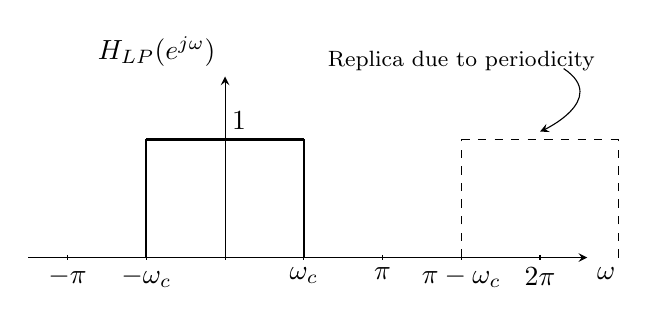
\begin{tikzpicture}
    \draw[-stealth] (-2.5,0) -- (4.6,0) node[anchor=north west] {$\omega$};
    \draw[-stealth] (0,0) -- (0,2.3) node[anchor=south east] {$H_{LP}(e^{j\omega})$};
    \draw[thick] (-1,0) -- (-1, 1.5) {};
    \draw[thick] (-1,1.5) -- (+1, 1.5) {};
    \draw[thick] (+1,0) -- (+1, 1.5) {};

    \draw[dashed] (-1+4,0) -- (-1+4, 1.5) {};
    \draw[dashed] (-1+4,1.5) -- (+1+4, 1.5) {};
    \draw[dashed] (+1+4,0) -- (+1+4, 1.5) {};

\foreach \x in {-2,-1,0,1,2,3,4}
    \draw (\x cm,1pt) -- (\x cm,-1pt) node[anchor=north] {};

    \draw (1 pt,1.5cm) -- (-1 pt,1.5cm) node[anchor=south west] {$1$};
    \node[anchor=north] at (-2,0) {$-\pi$};
    \node[anchor=north] at (-1,0) {$-\omega_c$};
    \node[anchor=north] at (+1,0) {$\omega_c$};
    \node[anchor=north] at (+2,0) {$\pi$};
    \node[anchor=north] at (+3,0) {$\pi - \omega_c$};
    \node[anchor=north] at (+4,0) {$2\pi$};

    \node[] at (+3, +2.5) {\footnotesize Replica due to periodicity};
    \draw[-stealth] (4.3,2.4) .. controls (4.9,2) and (4,1.6) .. (4,1.6);
\end{tikzpicture}
\end{center}

The inverse discrete-time Fourier Transform is soon obtained by
\begin{align*}
    h_{LP}[n] &= \int_{-\omega_c}^{\omega_c} e^{j\omega n}d\omega \\
              &= \frac 1 {2\pi} \left(\frac{e^{j\omega_c n}}{jn} - \frac{e^{-j\omega_c n}}{jn}\right)\\
              &= \frac {\sin {\omega_c n}}{\pi n}\\
              &= \sinc {\omega_c n}
\end{align*}
for all values $-\infty < n < \infty$.

For Parseval's Theorem, the energy of $h_{LP}[n]$ is given by $\frac {\omega_c}{\pi}$. Thus, $h_{LP}[n]$ is a finite-energy sequence, despite being \emph{not absolutely summable}. As a result, the quantity
\[
    \sum_{n=-K}^K h_{LP}[n] e^{-j\omega n} = \sum_{n=-K}^K \sinc {(\omega_c n)} e^{-j\omega n}
\]
does not uniformly converge to the Fourier Transform $H_{LP}(e^{j\omega)}$ for all $\omega$ values; still, it converges to $H_{LP}(e^{j\omega)}$ in the \emph{mean-square sense} because its energy is finite.

The mean-square convergence property of the sequence $h_{LP}[n]$ can be further illustrated bu examining the plot of the following function,
\[
    H_{LP,K}(e^{j\omega}) = \sum_{n=-K}^K e^{-j\omega n}\sinc {\omega_c n},
\]
for many values of $K$, as in Figure~\ref{tikz:discreteTimeFourierTransformExampleSinc}. A particularly interesting effect the Figure shows is the \textbf{Gibbs phenomenon}, a behavior of the DTFT in which multiple ripples---whose energy is smaller as the value of $K$ increases---are present. Verily, Gibbs phenomenon can be described as the oscillatory behavior of the Fourier series of a piecewise continuously differentiable periodic function around a jump discontinuity.
\begin{figure*}[ht]
\begin{center}
        \begin{tikzpicture}[
            declare function={fourier(\k,\x)=sin(0.4*\x*10 * \k)*(1/(3.1415*\k))*sin(-\x*0.4*10 *\k);}
            ]

                \begin{axis}[
                    at={(0,0)},
                    xlabel = $\omega$,
                    % ytick = {0,0.2,0.4,0.6,0.8,1},
                    %yticklabels = {$0.2$,$0.4$,$0.6$,$0.8$,$1$},
                    %xtick = {0,0.2,0.4,0.6,0.8,1},
                    %xticklabels = {$0$,$0.2$,$0.4$,$0.6$,$0.8$,$1$},
                    %ytick = {1},
                    %yticklabels = {1},
                    domain = 0:1,
                    samples = 200,
                    legend style = {%
                    at = {(0.5,1.02)},
                    anchor = south},
                    ]
                        \addlegendentry{$K=10$}
                            \addplot[mark = none, thick] gnuplot[raw gnuplot] {
                                set samples 200;
                                fourier(k, x) = 2*pi*sin(0.7*pi*k)*(1/(k*pi))*cos(0.7*pi*x*k);
                                plot[0:1] 0.7+ sum [k=1:10] 0.33*fourier(k,x+0.5);
                        };
                \end{axis};
\end{tikzpicture}
        \begin{tikzpicture}[
            declare function={fourier(\k,\x)=sin(0.4*\x*10 * \k)*(1/(3.1415*\k))*sin(-\x*0.4*10 *\k);}
            ]

                \begin{axis}[
                    at={(0,0)},
                    xlabel = $\omega$,
                    % ytick = {0,0.2,0.4,0.6,0.8,1},
                    %yticklabels = {$0.2$,$0.4$,$0.6$,$0.8$,$1$},
                    %xtick = {0,0.2,0.4,0.6,0.8,1},
                    %xticklabels = {$0$,$0.2$,$0.4$,$0.6$,$0.8$,$1$},
                    %ytick = {1},
                    %yticklabels = {1},
                    domain = 0:1,
                    samples = 200,
                    legend style = {%
                    at = {(0.5,1.02)},
                    anchor = south},
                    ]
                        \addlegendentry{$K=20$}
                            \addplot[mark = none, thick] gnuplot[raw gnuplot] {
                                set samples 200;
                                fourier(k, x) = 2*pi*sin(0.7*pi*k)*(1/(k*pi))*cos(0.7*pi*x*k);
                                plot[0:1] 0.7+ sum [k=1:20] 0.33*fourier(k,x+0.5);
                        };
                \end{axis};
            \node[] at (1.5, 6.5) {Gibbs phenomenon};
            \draw[-stealth] (1.5,6.4) .. controls (1.3,6) and (1.8,5.5) .. (1.7,5);
            \draw[-stealth] (2.9,6.5) .. controls (7,8) and (7,3.5) .. (5,1.2);
\end{tikzpicture}
\\
        \begin{tikzpicture}[
            declare function={fourier(\k,\x)=sin(0.4*\x*10 * \k)*(1/(3.1415*\k))*sin(-\x*0.4*10 *\k);}
            ]
                \begin{axis}[
                    at={(0,0)},
                    xlabel = $\omega$,
                    % ytick = {0,0.2,0.4,0.6,0.8,1},
                    %yticklabels = {$0.2$,$0.4$,$0.6$,$0.8$,$1$},
                    %xtick = {0,0.2,0.4,0.6,0.8,1},
                    %xticklabels = {$0$,$0.2$,$0.4$,$0.6$,$0.8$,$1$},
                    %ytick = {1},
                    %yticklabels = {1},
                    domain = 0:1,
                    samples = 200,
                    legend style = {%
                    at = {(0.5,1.02)},
                    anchor = south},
                    ]
                        \addlegendentry{$K=40$}
                            \addplot[mark = none, thick] gnuplot[raw gnuplot] {
                                set samples 200;
                                fourier(k, x) = 2*pi*sin(0.7*pi*k)*(1/(k*pi))*cos(0.7*pi*x*k);
                                plot[0:1] 0.7+ sum [k=1:40] 0.33*fourier(k,x+0.5);
                        };
                \end{axis};
\end{tikzpicture}
        \begin{tikzpicture}[
            declare function={fourier(\k,\x)=sin(0.4*\x*10 * \k)*(1/(3.1415*\k))*sin(-\x*0.4*10 *\k);}
            ]

                \begin{axis}[
                    at={(0,0)},
                    xlabel = $\omega$,
                    % ytick = {0,0.2,0.4,0.6,0.8,1},
                    %yticklabels = {$0.2$,$0.4$,$0.6$,$0.8$,$1$},
                    %xtick = {0,0.2,0.4,0.6,0.8,1},
                    %xticklabels = {$0$,$0.2$,$0.4$,$0.6$,$0.8$,$1$},
                    %ytick = {1},
                    %yticklabels = {1},
                    domain = 0:1,
                    samples = 400,
                    legend style = {%
                    at = {(0.5,1.02)},
                    anchor = south},
                    ]
                        \addlegendentry{$K=80$}
                            \addplot[mark = none, thick] gnuplot[raw gnuplot] {
                                set samples 400;
                                fourier(k, x) = 2*pi*sin(0.7*pi*k)*(1/(k*pi))*cos(0.7*pi*x*k);
                                plot[0:1] 0.7+ sum [k=1:80] 0.33*fourier(k,x+0.5);
                        };
                \end{axis};
\end{tikzpicture}
\end{center}\caption{Discrete-time Fourier Transform obtained through the mean-square convergence criterion. Noteworthy is the so called \emph{Gibbs phenomenon}, a sinusoidal effect that is always present in the DTFT and is manifest by means of a series of ripples in proximity of the magnitude change. The DTFT approximates an ideal \texttt{rect}.}\label{tikz:discreteTimeFourierTransformExampleSinc}
\end{figure*}
Ripples expressed by the Gibbs phenomenon are completely independent of $K$---the greater the $K$, the faster the oscillation will be. The number of ripples increases as $K$ increases, with the height of the largest ripple remaining the same for all values of $K$.

As $K$ goes to infinity, the integral condition
\[
    \lim_{K\rightarrow \infty}\int_{-\pi}^\pi \left|X(e^{j\omega}) - X_K(e^{j\omega})\right|^2 d\omega = 0
\]
holds indicating the convergence of $H_{LP,K}(e^{j\omega})$ towards $H_{LP}(e^{j\omega})$. The oscillatory behavior of $H_{LP,K}$ approximating the ``real'' DTFT in the mean-square sense is due to the Gibbs phenomenon.

The discrete-time Fourier Transform can also be defined for a specific class of sequences, which are neither absolutely summable nor square summable---a class of sequences whose energy is infinite. Examples of such sequences are the \emph{unit step sequence} $\mu[n]$, the sinusoidal sequence $\cos{(\omega_0 n + \varphi)}$ and the exponential sequence $A\alpha^n$. All of these possess infinite total energy and thus are not expressible by means of a ``standard'' DTFT.

In order to express infinite energy sequences with a discrete-time Fourier Transform, one has to adopt the \textbf{Dirac's delta function} $\delta(\omega)$. Dirac delta function is defined such as a function in $\omega$ with infinite height, zero-infinitesimal width, and unit area,
\begin{equation}\label{eqn:diracDelta}
    \lim_{\Delta\rightarrow 0} \int_{-\infty}^\infty p_\Delta(\omega)d\omega = \int_{-\infty}^\infty \delta(\omega)d\omega = 1.
\end{equation}
\begin{center}
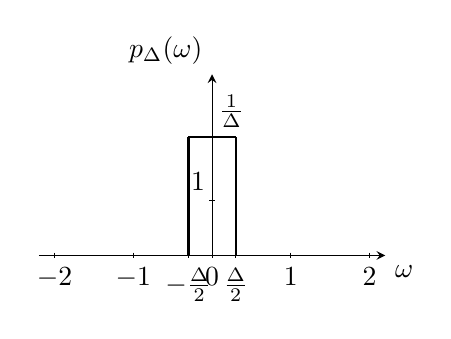
\begin{tikzpicture}
    \draw[-stealth] (-2.2,0) -- (2.2,0) node[anchor=north west] {$\omega$};
    \draw[-stealth] (0,0) -- (0,2.3) node[anchor=south east] {$p_\Delta(\omega)$};
    \draw[] (-1pt,0.7) -- (+1pt,0.7) node[anchor=south east] {$1$};
    \draw[thick] (-0.3,0) -- (-0.3, 1.5) {};
    \draw[thick] (-0.3,1.5) -- (+0.3, 1.5) {};
    \draw[thick] (+0.3,0) -- (0.3, 1.5) {};

\foreach \x in {-2,-1,0,1,2}
    \draw (\x cm,1pt) -- (\x cm,-1pt) node[anchor=north] {$\x$};

    \draw (1 pt,1.5cm) -- (-1 pt,1.5cm) node[anchor=south west] {$\frac 1 \Delta$};
    \draw (0.3 cm,1pt) -- (0.3 cm,-1pt) node[anchor=north] {$\frac \Delta 2$};
    \draw (-0.3 cm,1pt) -- (-0.3 cm,-1pt) node[anchor=north] {$-\frac \Delta 2$};

\end{tikzpicture}
\end{center}
The Dirac's delta is the limiting form of a unit area pulse function $p_\Delta(\omega)$ as $\Delta \rightarrow 0$, satisfying Equation~\ref{eqn:diracDelta}.

As an exaple, consider the complex exponential sequence
\begin{equation}\label{eqn:complexExponentialSequence}
    x[n] = e^{j \omega_0 n}.
\end{equation}
Its discrete-time Fourier Transform is given by the following
\begin{equation}\label{eqn:complexExponentialSequenceFourierTransform}
    X(e^{j\omega}) = \sum_{k=-\infty}^\infty 2\pi \delta(\omega - \omega_0 + 2\pi k)
\end{equation}
with $\delta(\omega)$ being the Dirac's delta impulse function and $-\pi \leq \omega_0 \leq \pi$. The function expressed by~\ref{eqn:complexExponentialSequenceFourierTransform} is a periodic function of $\omega$---this can be seen by the $2\pi k$ term in the Dirac's delta argument---which has a peculiar name and is called \emph{periodic impulse train}. To verify that the above DTFT is the correct one, the best idea would be to simply compute the inverse discrete-time Fourier Transform of $X(e^{j\omega})$. Therefore,
\begin{align*}
    x[n] &= \frac 1 {2\pi} \int_{-\pi}^\pi \sum_{k=-\infty}^\infty 2\pi\delta(\omega - \omega_0 + 2\pi k)e^{j\omega n}d\omega\\
         &= \int_{-\pi}^\pi \delta(\omega - \omega_0) e^{j\omega n} d\omega = e^{j\omega_0 n},
\end{align*}
where we have employed the sampling property of the impulse function\footnote{
    The sampling property of the impulse function is different regarding of the discrete or continuous domain, and states that
    \begin{equation}\label{eqn:samplingPropertyDeltaSum}
        \sum_{k=-\infty}^\infty e^{j2\pi n}\delta(n-k) = e^{j 2 \pi k},
    \end{equation}
    and
    \begin{equation}\label{eqn:samplingPropertyDeltaIntegral}
        \int_{-\infty}^\infty \delta(\omega-\omega_0)e^{j\omega} = e^{j\omega_0}.
    \end{equation}
} $\delta(\omega)$.

This way, one can define numerous commonly used DTFT pairs, such as the following ones,
\[
    \begin{array}{rcl}
        \delta[n] & \longleftrightarrow & 1, \\
        1 & \longleftrightarrow & \sum_{k=-\infty}^\infty 2\pi \delta(\omega + 2\pi k), \\
        1\cdot e^{j\omega_0 n} & \longleftrightarrow & \sum_{k=-\infty}^\infty 2\pi \delta(\omega - \omega_0 + 2\pi k), \\
        \mu[n] & \longleftrightarrow & \frac {1}{1 - e^{-j\omega}} + \sum_{k=-\infty}^\infty \pi \delta(\omega + 2\pi k), \\
        \alpha^n \mu[n], (|\alpha| < 1) & \longleftrightarrow & \frac{1}{1 - \alpha e^{-j\omega}}.
    \end{array}
\]
The last equation, in particular, depends on a parameter $\alpha$: if $|\alpha| \geq 1$ then a representation like the above cannot be employed, and instead one is forced to employ Dirac's delta impulses.
\clearpage

\subsection{List of noteworthy discrete-time Fourier Transform Theorems and formulas}

\begin{table*}[ht]
\centering
\begin{tabular}{c c}
    \hline
    \textbf{Sequence} & \textbf{Discrete-time Fourier Transform} \\
    \hline
    $x[n]$ (a complex sequence) & $X(e^{j\omega})$ \\
    \hline
    $x[-n]$ & $X(e^{-j\omega})$ \\
    $x^*[n]$ & $X^*(e^{j\omega})$ \\
    $\Re{\{x[n]\}}$ & $X_{cs}(e^{j\omega}) = \frac 1 2 \{X(e^{j\omega}) + X^*(e^{-j\omega})\}$\\
    $j\Im{\{x[n]\}}$ & $X_{ca}(e^{j\omega}) = \frac 1 2 \{X(e^{j\omega}) - X^*(e^{-j\omega})\}$\\
    $x_{cs}[n]$ & $X_{re}(e^{j\omega})$ \\
    $x_{ca}[n]$ & $jX_{im}(e^{j\omega})$ \\
    \hline
\end{tabular}
\caption{Notable discrete-time Fourier Transform properties. $X_{cs}(e^{j\omega})$ and $X_{ca}(e^{j\omega})$ are the conjugate-symmetric and conjugate-antisymmetric parts of $X(e^{j\omega})$, respectively. Likewise, $x_{cs}[n]$ and $x_{ca}[n]$ are, respectively, the conjugate-symmetric and conjugate-antisymmetric parts of $x[n]$.}\label{tab:discreteTimeFourierTransformPropertiesAndTheorems}
\end{table*}

\begin{table*}[ht]
\centering
\begin{tabular}{c c}
    \hline
    \textbf{Sequence} & \textbf{Discrete-time Fourier Transform} \\
    \hline
    $x[n]$ & $X(e^{j\omega}) = X_{re}(e^{j\omega)} + jX_{im}(e^{j\omega)}$ \\
    \hline
    $x_{ev}[n]$ & $X_{re}(e^{j\omega})$ \\
    $x_{od}[n]$ & $jX_{im}(e^{j\omega})$ \\
    \hline
    Symmetry relations & $X(e^{j\omega}) = X^*(e^{-j\omega})$ \\
    --- & $X_{re}(e^{j\omega}) = X_{re}(e^{-j\omega})$ \\
    --- & $X_{im}(e^{j\omega}) = -X_{im}(e^{-j\omega})$ \\
    --- & $|X(e^{j\omega})| = |X(e^{-j\omega})|$ \\
    --- & $\arg{X(e^{j\omega})} = -\arg{X(e^{-j\omega})}$ \\
    \hline
\end{tabular}
\caption{Notable discrete-time Fourier Transform properties. Sequences $x_{ev}[n]$ and $x_{od}[n]$ are, respectively, the even and the odd parts of the sequence $x[n]$.}\label{tab:discreteTimeFourierTransformPropertiesAndTheorems2}
\end{table*}

\begin{table*}[ht]
\centering
\begin{tabular}{ccc}
    \hline
    \textbf{Name} & \textbf{Sequence} & \textbf{Discrete-time Fourier Transform} \\
    \hline
    Linearity & $\alpha g[n] + \beta h[n]$ & $\alpha G(e^{j\omega}) + \beta H(e^{j\omega})$\\
    Time-shifting & $g[n-n_0]$ & $e^{-j\omega n_0} G(e^{j\omega})$ \\
    Frequency-shifting & $e^{j\omega_0 n}g[n]$ & $G\left((e^{j(\omega - \omega_0)}\right)$ \\
    Frequency differentiation & $ng[n]$ & $j\frac {dG(e^{j\omega})}{d\omega}$ \\
    Convolution & $g[n] \circledast h[n]$ &$ G(e^{j\omega}) \cdot H(e^{j\omega})$\\
    Modulation & $g[n] \cdot h[n]$ &$ \frac{1}{2\pi} \int_{-\pi}^\pi G(e^{j\theta}) \cdot H(e^{j(\omega - \theta)}) d\theta$\\
    \hline
    Parseval's relation & $\sum_{n=-\infty}^\infty g[n]h^*[n]$ &$= \frac 1 {2\pi} \int_{-\pi}^\pi G(e^{j\omega})H^*(e^{j\omega})d\omega$\\
    \hline
\end{tabular}
\caption{Notable discrete-time Fourier Transform properties.}\label{tab:discreteTimeFourierTransformPropertiesAndTheorems3}
\end{table*}

A number of important properties and theorems, very useful in digital signal processing applications, are listed without proof in Tables~\ref{tab:discreteTimeFourierTransformPropertiesAndTheorems}, \ref{tab:discreteTimeFourierTransformPropertiesAndTheorems2} and~\ref{tab:discreteTimeFourierTransformPropertiesAndTheorems3}.


For instance, suppose to find the DTFT $V(e^{j\omega})$ of a sequence $v[n]$ that follows the relationship
\[d_0 v[n] + d_1v[n-1] = p_0 \delta[n] + p_1\delta[n-1].\]
The discrete-time Fourier Transform of the delta impulse is exactly $1$---using the time-shifting theorem of the DTFT given by Table~\ref{tab:discreteTimeFourierTransformPropertiesAndTheorems3} one finds that the DTFT of $\delta[n-1]$ is $e^{-j\omega}$, and the DTFT of $v[n-1]$ is $e^{-j\omega}V(e^{j\omega})$. Applying the linearity theorem from the same Table, one gets the frequency-domain representation
\[
\begin{array}{ccccccc}
    d_0v[n] &+& d_1v[n-1] &=& p_0\delta[n] &+& p_1\delta[n-1]\\
    \updownarrow & & \updownarrow & & \updownarrow & & \updownarrow \\
    d_0V(e^{j\omega} &+& d_1e^{-j\omega}V(e^{j\omega}) &=& p_0 &+& p_1e^{-j\omega}.
\end{array}
\]

By solving the above equation, one obtains the final formula
\[
    V(e^{j\omega}) = \frac{p_0 + p_1 e^{-j\omega}}{d_0 + d_1e^{-j\omega}}.
\]

\section{Energy Density Spectrum relationshipts in discrete-time Fourier Transforms}

Let $g[n]$ be a \emph{finite-energy} sequence. We have already seen that the total energy of $g[n]$ is the quantity
\[
    \mathcal E_x = \sum_{n=-\infty}^\infty | g[n]|^2.
\]

From the Pareseval's theorem in Table~\ref{tab:discreteTimeFourierTransformPropertiesAndTheorems3} one can soon observe that
\begin{equation}\label{eqn:energyDensitySpectrumParseval}
    \mathcal E_x = \sum_{n=-\infty}^\infty | g[n]|^2 = \frac 1{2\pi} \int_{-\pi}^\pi \underbrace{\left|G(e^{j\omega})\right|^2}_{S_{gg}(\omega)} d\omega.
\end{equation}
where the quantity $S_{gg}(\omega) = \left|G(e^{j\omega})\right|^2$ is called energy density spectrum, as in Equation~\ref{eqn:energyDensitySpectrum}.

The energy density spectrum draws a curve---the area under the curve in the frequency range $-\pi < \omega \leq \pi$ divided by $2\pi$ is called \textbf{Area Under the Curve}.

Spectrum of signals will differ in relation to their band type.

Since the spectrum of a discrete-time signal is a periodic function of $\omega$ having period $2\pi$, a \emph{full-band} signal will possess a spectrum lying in the whole frequency range of $-\pi < \omega \leq \pi$. Vice-versa, a \emph{band-limited} discrete-time signal will possess a spectrum which will be limited to a specific portion of the frequency range $-\pi < \omega \leq \pi$.

Any \emph{ideal band-limited} signal has a spectrum that is zero outside a specific frequency range $[\omega_a, \omega_b]$, that is indeed expressed in Equation~\ref{eqn:idealBandSignal},
\[
    X(j\omega) = \left\{\begin{array}{ll}
        0,  &   0 \leq |\omega| \leq \omega_a\\
        0,  &   \omega_b \leq |\omega| \leq \infty\\
        X(j\omega)  &   \omega_a \leq |\omega| \leq \omega_b
    \end{array}\right..
\]

In Section~\ref{sec:bandLimitedSignals} we have already encountered \emph{lowpass}, \emph{highpass} and \emph{bandpass} signals. To recap,
\begin{description}
    \item[Lowpass] signals are all signals arranged in a frequency range $|\omega| \leq \omega_p < \infty$, where $\omega_p$ is said to be the \emph{bandwidth} of the signal;
    \item[Highpass] signals are all signals arranged in a frequency range $0 < \omega_p \leq |\omega| < \infty$, where the bandwitdh of the signal is in the interval $[\omega_p, \infty[$.
    \item[Bandpass] signals are any signal whose spectrum is located in the frequency range $[\omega_L, \omega_H]$, that is $0 < \omega_L \leq |\omega| \leq \omega_H < \infty$, where the bandwidth is given by $\mathrm{BW} = \omega_H - \omega_L$.
\end{description}

Consider as an example the sequence \[x[n] = (0.5)^n \mu[n];\] its discrete-time Fourier Transform is given below on the left along with its \emph{magnitude spectrum} shown below.
\begin{center}
    \begin{tikzpicture}[
        ]
            \begin{axis}[
                at={(0,0)},
                xlabel = $\frac \omega \pi$,
                % ytick = {0,0.2,0.4,0.6,0.8,1},
                %yticklabels = {$0.2$,$0.4$,$0.6$,$0.8$,$1$},
                %xtick = {0,0.2,0.4,0.6,0.8,1},
                %xticklabels = {$0$,$0.2$,$0.4$,$0.6$,$0.8$,$1$},
                %ytick = {1},
                %yticklabels = {1},
                domain = 0:1,
                samples = 200,
                legend style = {%
                at = {(0.5,1.02)},
                anchor = south},
                ]
                \addlegendentry{$|X(e^{j\omega})|$}
                        \addplot[mark = none, thick] gnuplot[raw gnuplot] {
                            set samples 200;
                            magnitude(x) = 1/(1-0.5*cos(pi*x));
                            d(x) = sqrt(1 - 2*0.5*cos(pi*x) + (0.5)^2);
                            magnitude(x) = 1/(d(x));
                            plot[+0:1] magnitude(x);
                    };
                \addlegendentry{$b_{80}$}
                        \addplot+[mark = none, draw=red] gnuplot[raw gnuplot] {
                            magnitude(x) = 1/(1-0.5*cos(pi*x));
                            d(x) = sqrt(1 - 2*0.5*cos(pi*x) + (0.5)^2);
                            magnitude(x) = 1/(d(x));
                            set parametric;
                            plot [t=+0.5:magnitude(0.5081)] 0.5081,t;
                    };
            \end{axis};
    \end{tikzpicture}
\end{center}


It can be shown that the $80\%$ of the energy of the lowpass signal in the above example is contained in a very precise frequency range, that is $0 \leq |\omega| \leq 0.5081\pi$. Therefore, we can define the \emph{$80\%$ bandwidth frequency} as the frequency $b_{80} = 0.5081\pi$.

In another example one has the sequence
\[
    h_{LP}[n] = \frac {\sin {\omega_c n}}{\pi n}.
\]

In order to compute the total energy one uses the Parseval's theorem as follows,
\[
h_{LP}[n] = \sum_{n=-\infty}^\infty \left|h_{LP}[n]\right|^2 = \frac 1 {2\pi} \int_{-\pi}^\pi \left|H_{LP}(e^{j\omega})\right|^2d\omega,
\]
where the already known discrete-time Fourier Transform $H_{LP}(e^{j\omega})$ is the function
\[
    H_{LP}(e^{j\omega}) = \left\{\begin{array}{ll}
        1 & 0 \leq |\omega| \leq \omega_c\\
        0 & \omega_c \leq |\omega| \leq \pi
        \end{array}\right..
\]

By applying the latter in the Parseval's theorem equation, one finally gets
\[
h_{LP}[n] = \sum_{n=-\infty}^\infty \left|h_{LP}[n]\right|^2 = \frac 1 {2\pi} \int_{-\omega_c}^{\omega_c} d\omega = \frac {\omega_c} \pi < \infty,
\]
showing that the sequence $h_{LP}[n]$ is a lowpass sequence possessing finite energy.


In \textsc{Matlab}, the function \texttt{freqz} can be invoked to compute the values of the discrete-time Fourier Transform of a sequence, described as a rational function having the form
\begin{equation}\label{eqn:dtftRationalForm}
    X(e^{j\omega}) = \frac
    {p_0 + p_1e^{-j\omega} + \dots + p_m e^{-j\omega m}}
    {d_0 + d_1e^{-j\omega} + \dots + d_n e^{-j\omega n}},
\end{equation}
at a prescribed set of discrete frequency points $\omega = \omega_l$, dense enough to \emph{look} continuous\footnote{Indeed, no calculator can possibly compute all the infinite points of the continuous curve, and can only determine the values of the transform for a finite number of them.}.

The statement
\begin{verbatim}
H = freqz(num, den, w);
\end{verbatim}
instructs \textsc{Matlab} to return the frequency response values of a discrete-time Fourier Transform defined in terms of the vectors \texttt{num} and \texttt{den}, con\-tain\-ing---res\-pec\-ti\-ve\-ly---the coefficients $\{p_i\}$ and $\{d_i\}$, at a prescribed set of frequencies between $0$ and $2\pi$ given by the vector \texttt{w}. The result is returned as a vector \texttt{H}.

As an example, let's plot the real and imaginary parts along with the magnitude and phase spectra of the following discrete-time Fourier Transform,
\begin{equation}\label{eqn:octaveExampleFreqz}
    X(e^{j\omega}) = \frac
    {0.008 - 0.033e^{-j\omega} + 0.05e^{-j2\omega} - 0.033e^{-j3\omega} + 0.008e^{-j4\omega}}
    {1 + 2.37e^{-j\omega} + 2.7e^{-j2\omega} + 1.6e^{-j3\omega} + 0.4e^{-j4\omega}}
\end{equation}

First off, let's define the proper variables,
\begin{verbatim}
pkg load signal;
num = [0.008 -0.033 0.05 -0.033 0.008];
den = [1 2.37 2.7 1.6 0.4];
w = [0:0.01:3.14];
\end{verbatim}
and then compute the DTFT as we have seen,
\begin{verbatim}
H = freqz(num, den, w);
\end{verbatim}

A quick plot, for instance, of the real part can be quickly produced with
\begin{verbatim}
plot(w, real(H));
\end{verbatim}
however, plots as in Figure~\ref{oct:octaveExampleFreqz} have been generated with the \texttt{subplot} command,
\begin{verbatim}
set(groot,'defaultLineLineWidth',2.0)
figure(1);
subplot(2, 2, 1); plot(w, real(H));
title("Real part of H");
subplot(2, 2, 2); plot(w, imag(H));
title("Imaginary part of H");
subplot(2, 2, 3); plot(w, abs(H));
title("Magnitude spectrum of H");
subplot(2, 2, 4); plot(w, angle(H));
title("Phase spectrum of H");
\end{verbatim}
which were enough to generate the four-plot grid.

% print -depslatex -mono "-S800,600" "figure-name.tex"
\begin{figure}[ht]
    \begin{center}
\scalebox{0.6}{
% Title: gl2ps_renderer figure
% Creator: GL2PS 1.4.2, (C) 1999-2020 C. Geuzaine
% For: Octave
% CreationDate: Tue Oct 18 17:09:43 2022
\setlength{\unitlength}{1pt}
\begin{picture}(0,0)
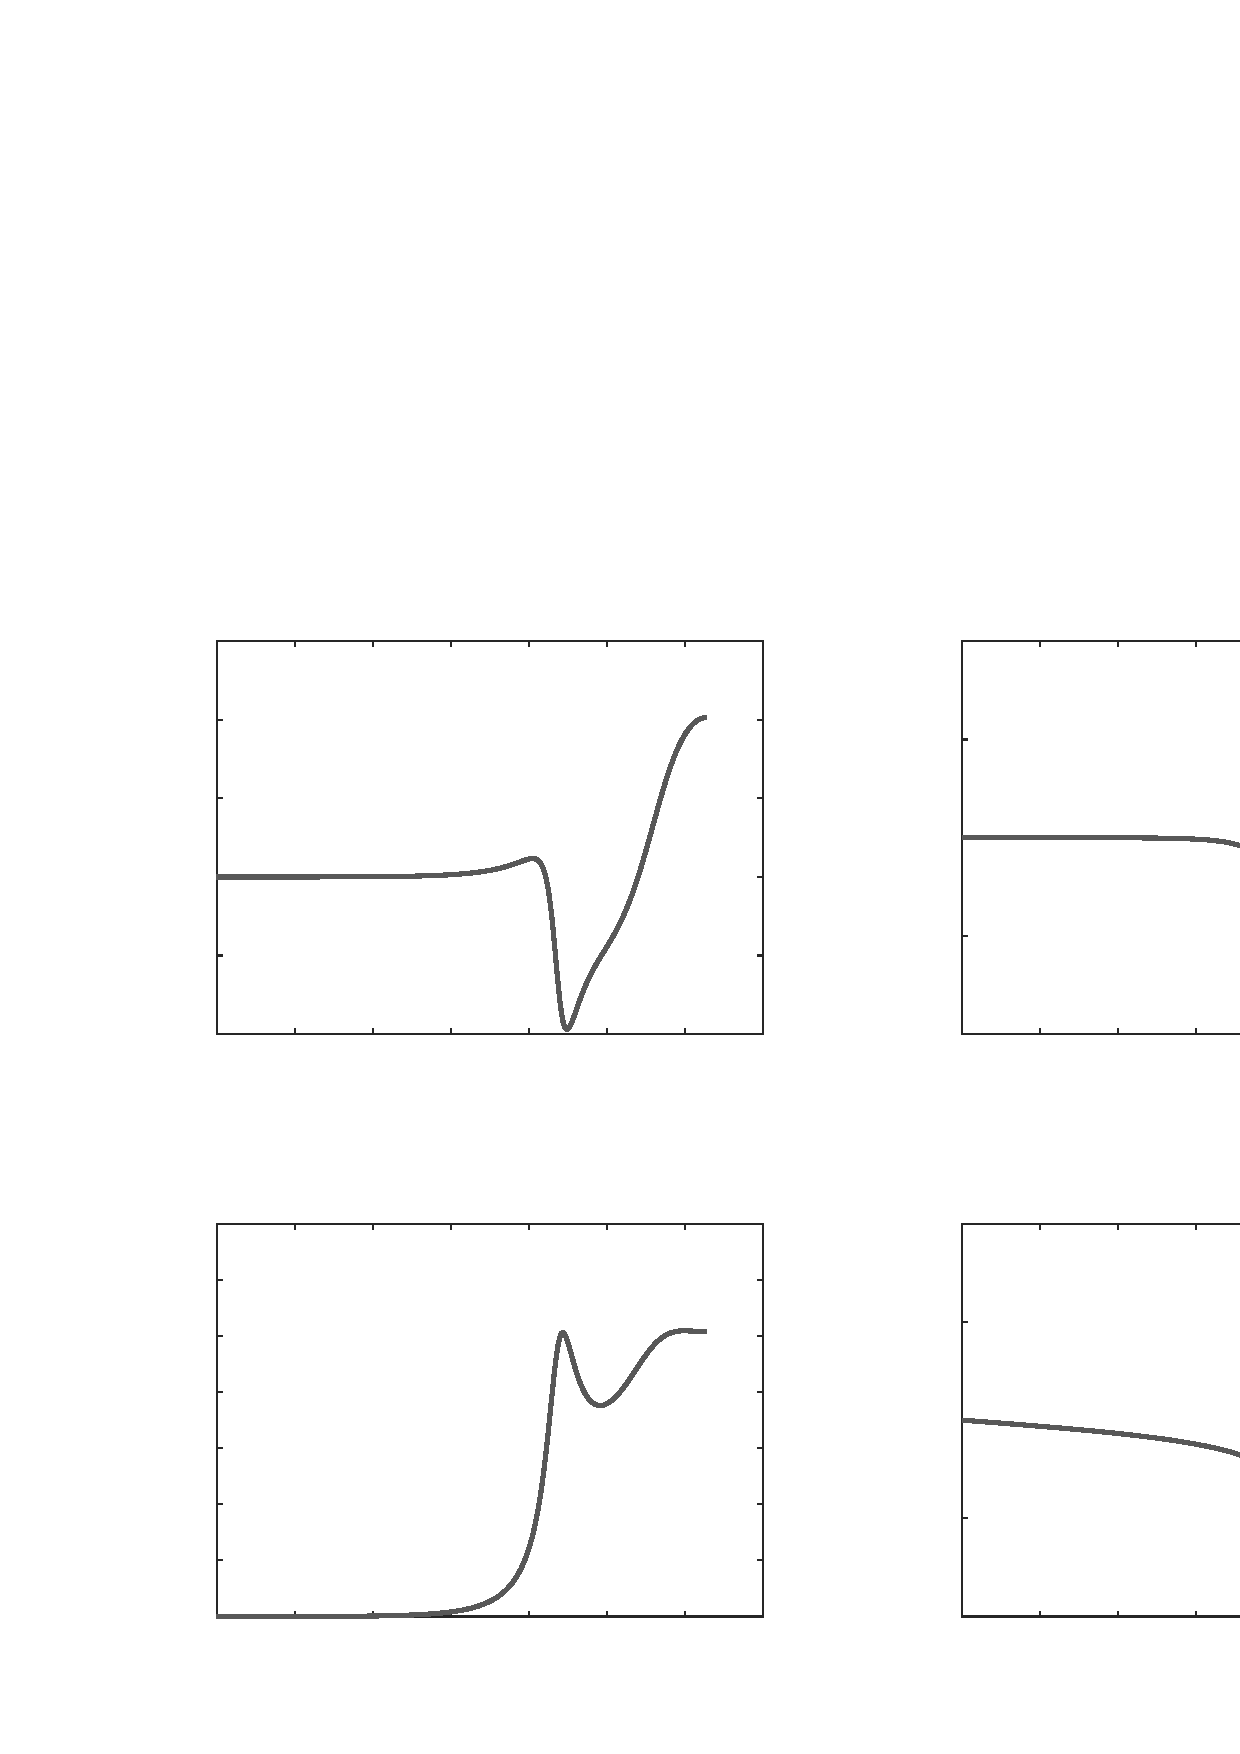
\includegraphics[scale=1]{octaves/dtft-example-inc}
\end{picture}%
\begin{picture}(800,600)(0,0)
\fontsize{13}{0}\selectfont\put(104,335.128){\makebox(0,0)[t]{\textcolor[rgb]{0.15,0.15,0.15}{{0}}}}
\fontsize{13}{0}\selectfont\put(141.438,335.128){\makebox(0,0)[t]{\textcolor[rgb]{0.15,0.15,0.15}{{0.5}}}}
\fontsize{13}{0}\selectfont\put(178.875,335.128){\makebox(0,0)[t]{\textcolor[rgb]{0.15,0.15,0.15}{{1}}}}
\fontsize{13}{0}\selectfont\put(216.313,335.128){\makebox(0,0)[t]{\textcolor[rgb]{0.15,0.15,0.15}{{1.5}}}}
\fontsize{13}{0}\selectfont\put(253.75,335.128){\makebox(0,0)[t]{\textcolor[rgb]{0.15,0.15,0.15}{{2}}}}
\fontsize{13}{0}\selectfont\put(291.188,335.128){\makebox(0,0)[t]{\textcolor[rgb]{0.15,0.15,0.15}{{2.5}}}}
\fontsize{13}{0}\selectfont\put(328.625,335.128){\makebox(0,0)[t]{\textcolor[rgb]{0.15,0.15,0.15}{{3}}}}
\fontsize{13}{0}\selectfont\put(366.063,335.128){\makebox(0,0)[t]{\textcolor[rgb]{0.15,0.15,0.15}{{3.5}}}}
\fontsize{13}{0}\selectfont\put(97.0508,345.577){\makebox(0,0)[r]{\textcolor[rgb]{0.15,0.15,0.15}{{-1}}}}
\fontsize{13}{0}\selectfont\put(97.0508,383.277){\makebox(0,0)[r]{\textcolor[rgb]{0.15,0.15,0.15}{{-0.5}}}}
\fontsize{13}{0}\selectfont\put(97.0508,420.977){\makebox(0,0)[r]{\textcolor[rgb]{0.15,0.15,0.15}{{0}}}}
\fontsize{13}{0}\selectfont\put(97.0508,458.677){\makebox(0,0)[r]{\textcolor[rgb]{0.15,0.15,0.15}{{0.5}}}}
\fontsize{13}{0}\selectfont\put(97.0508,496.377){\makebox(0,0)[r]{\textcolor[rgb]{0.15,0.15,0.15}{{1}}}}
\fontsize{13}{0}\selectfont\put(97.0508,534.077){\makebox(0,0)[r]{\textcolor[rgb]{0.15,0.15,0.15}{{1.5}}}}
\fontsize{15}{0}\selectfont\put(235.032,544.077){\makebox(0,0)[b]{\textcolor[rgb]{0,0,0}{{Real part of H}}}}
\fontsize{13}{0}\selectfont\put(461.937,335.128){\makebox(0,0)[t]{\textcolor[rgb]{0.15,0.15,0.15}{{0}}}}
\fontsize{13}{0}\selectfont\put(499.375,335.128){\makebox(0,0)[t]{\textcolor[rgb]{0.15,0.15,0.15}{{0.5}}}}
\fontsize{13}{0}\selectfont\put(536.812,335.128){\makebox(0,0)[t]{\textcolor[rgb]{0.15,0.15,0.15}{{1}}}}
\fontsize{13}{0}\selectfont\put(574.25,335.128){\makebox(0,0)[t]{\textcolor[rgb]{0.15,0.15,0.15}{{1.5}}}}
\fontsize{13}{0}\selectfont\put(611.687,335.128){\makebox(0,0)[t]{\textcolor[rgb]{0.15,0.15,0.15}{{2}}}}
\fontsize{13}{0}\selectfont\put(649.125,335.128){\makebox(0,0)[t]{\textcolor[rgb]{0.15,0.15,0.15}{{2.5}}}}
\fontsize{13}{0}\selectfont\put(686.562,335.128){\makebox(0,0)[t]{\textcolor[rgb]{0.15,0.15,0.15}{{3}}}}
\fontsize{13}{0}\selectfont\put(724,335.128){\makebox(0,0)[t]{\textcolor[rgb]{0.15,0.15,0.15}{{3.5}}}}
\fontsize{13}{0}\selectfont\put(454.988,345.577){\makebox(0,0)[r]{\textcolor[rgb]{0.15,0.15,0.15}{{-1}}}}
\fontsize{13}{0}\selectfont\put(454.988,392.702){\makebox(0,0)[r]{\textcolor[rgb]{0.15,0.15,0.15}{{-0.5}}}}
\fontsize{13}{0}\selectfont\put(454.988,439.827){\makebox(0,0)[r]{\textcolor[rgb]{0.15,0.15,0.15}{{0}}}}
\fontsize{13}{0}\selectfont\put(454.988,486.952){\makebox(0,0)[r]{\textcolor[rgb]{0.15,0.15,0.15}{{0.5}}}}
\fontsize{13}{0}\selectfont\put(454.988,534.077){\makebox(0,0)[r]{\textcolor[rgb]{0.15,0.15,0.15}{{1}}}}
\fontsize{15}{0}\selectfont\put(592.969,544.077){\makebox(0,0)[b]{\textcolor[rgb]{0,0,0}{{Imaginary part of H}}}}
\fontsize{13}{0}\selectfont\put(104,55.551){\makebox(0,0)[t]{\textcolor[rgb]{0.15,0.15,0.15}{{0}}}}
\fontsize{13}{0}\selectfont\put(141.438,55.551){\makebox(0,0)[t]{\textcolor[rgb]{0.15,0.15,0.15}{{0.5}}}}
\fontsize{13}{0}\selectfont\put(178.875,55.551){\makebox(0,0)[t]{\textcolor[rgb]{0.15,0.15,0.15}{{1}}}}
\fontsize{13}{0}\selectfont\put(216.313,55.551){\makebox(0,0)[t]{\textcolor[rgb]{0.15,0.15,0.15}{{1.5}}}}
\fontsize{13}{0}\selectfont\put(253.75,55.551){\makebox(0,0)[t]{\textcolor[rgb]{0.15,0.15,0.15}{{2}}}}
\fontsize{13}{0}\selectfont\put(291.188,55.551){\makebox(0,0)[t]{\textcolor[rgb]{0.15,0.15,0.15}{{2.5}}}}
\fontsize{13}{0}\selectfont\put(328.625,55.551){\makebox(0,0)[t]{\textcolor[rgb]{0.15,0.15,0.15}{{3}}}}
\fontsize{13}{0}\selectfont\put(366.063,55.551){\makebox(0,0)[t]{\textcolor[rgb]{0.15,0.15,0.15}{{3.5}}}}
\fontsize{13}{0}\selectfont\put(97.0508,66){\makebox(0,0)[r]{\textcolor[rgb]{0.15,0.15,0.15}{{0}}}}
\fontsize{13}{0}\selectfont\put(97.0508,92.9285){\makebox(0,0)[r]{\textcolor[rgb]{0.15,0.15,0.15}{{0.2}}}}
\fontsize{13}{0}\selectfont\put(97.0508,119.857){\makebox(0,0)[r]{\textcolor[rgb]{0.15,0.15,0.15}{{0.4}}}}
\fontsize{13}{0}\selectfont\put(97.0508,146.786){\makebox(0,0)[r]{\textcolor[rgb]{0.15,0.15,0.15}{{0.6}}}}
\fontsize{13}{0}\selectfont\put(97.0508,173.714){\makebox(0,0)[r]{\textcolor[rgb]{0.15,0.15,0.15}{{0.8}}}}
\fontsize{13}{0}\selectfont\put(97.0508,200.643){\makebox(0,0)[r]{\textcolor[rgb]{0.15,0.15,0.15}{{1}}}}
\fontsize{13}{0}\selectfont\put(97.0508,227.571){\makebox(0,0)[r]{\textcolor[rgb]{0.15,0.15,0.15}{{1.2}}}}
\fontsize{13}{0}\selectfont\put(97.0508,254.5){\makebox(0,0)[r]{\textcolor[rgb]{0.15,0.15,0.15}{{1.4}}}}
\fontsize{15}{0}\selectfont\put(235.032,264.5){\makebox(0,0)[b]{\textcolor[rgb]{0,0,0}{{Magnitude spectrum of H}}}}
\fontsize{13}{0}\selectfont\put(461.937,55.6063){\makebox(0,0)[t]{\textcolor[rgb]{0.15,0.15,0.15}{{0}}}}
\fontsize{13}{0}\selectfont\put(499.375,55.6063){\makebox(0,0)[t]{\textcolor[rgb]{0.15,0.15,0.15}{{0.5}}}}
\fontsize{13}{0}\selectfont\put(536.812,55.6063){\makebox(0,0)[t]{\textcolor[rgb]{0.15,0.15,0.15}{{1}}}}
\fontsize{13}{0}\selectfont\put(574.25,55.6063){\makebox(0,0)[t]{\textcolor[rgb]{0.15,0.15,0.15}{{1.5}}}}
\fontsize{13}{0}\selectfont\put(611.687,55.6063){\makebox(0,0)[t]{\textcolor[rgb]{0.15,0.15,0.15}{{2}}}}
\fontsize{13}{0}\selectfont\put(649.125,55.6063){\makebox(0,0)[t]{\textcolor[rgb]{0.15,0.15,0.15}{{2.5}}}}
\fontsize{13}{0}\selectfont\put(686.562,55.6063){\makebox(0,0)[t]{\textcolor[rgb]{0.15,0.15,0.15}{{3}}}}
\fontsize{13}{0}\selectfont\put(724,55.6063){\makebox(0,0)[t]{\textcolor[rgb]{0.15,0.15,0.15}{{3.5}}}}
\fontsize{13}{0}\selectfont\put(454.988,66){\makebox(0,0)[r]{\textcolor[rgb]{0.15,0.15,0.15}{{-4}}}}
\fontsize{13}{0}\selectfont\put(454.988,113.125){\makebox(0,0)[r]{\textcolor[rgb]{0.15,0.15,0.15}{{-2}}}}
\fontsize{13}{0}\selectfont\put(454.988,160.25){\makebox(0,0)[r]{\textcolor[rgb]{0.15,0.15,0.15}{{0}}}}
\fontsize{13}{0}\selectfont\put(454.988,207.375){\makebox(0,0)[r]{\textcolor[rgb]{0.15,0.15,0.15}{{2}}}}
\fontsize{13}{0}\selectfont\put(454.988,254.5){\makebox(0,0)[r]{\textcolor[rgb]{0.15,0.15,0.15}{{4}}}}
\fontsize{15}{0}\selectfont\put(592.969,264.5){\makebox(0,0)[b]{\textcolor[rgb]{0,0,0}{{Phase spectrum of H}}}}
\end{picture}

}\caption{\emph{Real part}, \emph{imaginary part}, \emph{magnitude spectrum} and \emph{phase spectrum} plots of Example~\ref{eqn:octaveExampleFreqz}. Notice the discontinuity in the $\arctan{}$ function that manifests with a sudden jump in the phase spectrum. Plots have been generated with the help of \texttt{octave}.}\label{oct:octaveExampleFreqz}
    \end{center}
\end{figure}
\clearpage

\subsection{The Unwrapped Phase Function}
In numerical computation when the computed phase function is outside of the possible range of $\omega$---that is $[-\pi, \pi]$---to bring the computed value to the correct range the phase is computed \emph{modulo} $2\pi$. Hence, the phase may exhibit some discontinuities of $2\pi$ radians in the phase spectrum plot, as in Figure~\ref{oct:octaveExampleFreqz}. Indeed, one would like to possess some kind of representation which doesn't present any kind of visible discontinuity; to do so, one should adopt the \textbf{unwrapped phase function}.

Unwrapped phase functions are special functions whose goal is to represent the phase without any dis\-con\-ti\-nui\-ty---that is, by \emph{unwrapping the phase}. Related function goes under the name of $\theta_c(\omega)$. In the following Figure~\ref{oct:octaveExampleFreqzUnwrap} the unwrapped phase spectrum has been plotted with the commands
\begin{verbatim}
plot(w,unwrap(angle(H)));
\end{verbatim}
which are enough to produce a plot of the desired unwrapped phase function of \texttt{H}.

% print -depslatex -mono "-S800,600" "figure-name.tex"
\begin{figure}[ht]
    \begin{center}
\scalebox{0.6}{
% Title: gl2ps_renderer figure
% Creator: GL2PS 1.4.2, (C) 1999-2020 C. Geuzaine
% For: Octave
% CreationDate: Wed Oct 19 08:41:45 2022
\setlength{\unitlength}{1pt}
\begin{picture}(0,0)
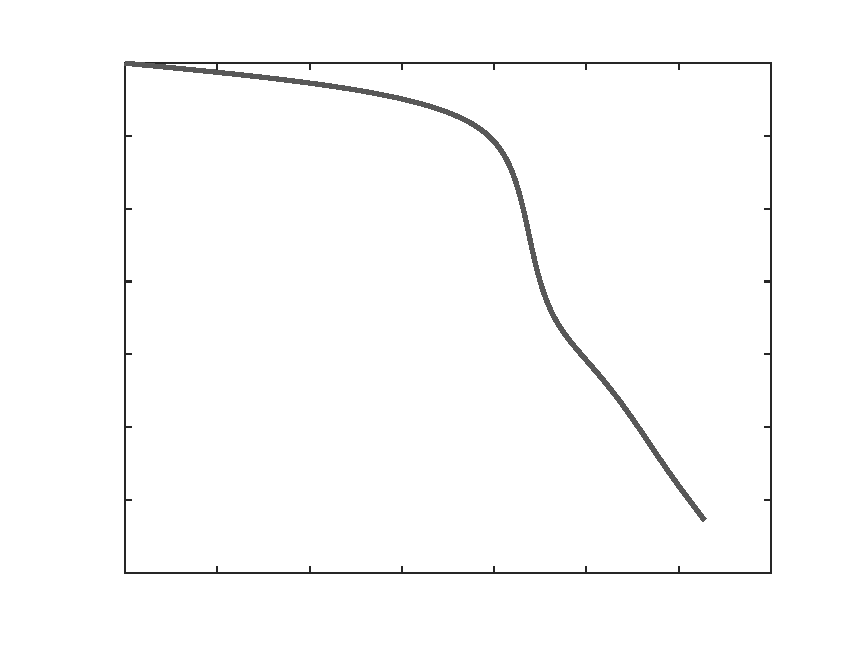
\includegraphics[scale=1]{octaves/dtft-unwrap-inc}
\end{picture}%
\begin{picture}(400,300)(0,0)
\fontsize{6}{0}\selectfont\put(52,27.7787){\makebox(0,0)[t]{\textcolor[rgb]{0.15,0.15,0.15}{{0}}}}
\fontsize{6}{0}\selectfont\put(96.2857,27.7787){\makebox(0,0)[t]{\textcolor[rgb]{0.15,0.15,0.15}{{0.5}}}}
\fontsize{6}{0}\selectfont\put(140.571,27.7787){\makebox(0,0)[t]{\textcolor[rgb]{0.15,0.15,0.15}{{1}}}}
\fontsize{6}{0}\selectfont\put(184.857,27.7787){\makebox(0,0)[t]{\textcolor[rgb]{0.15,0.15,0.15}{{1.5}}}}
\fontsize{6}{0}\selectfont\put(229.143,27.7787){\makebox(0,0)[t]{\textcolor[rgb]{0.15,0.15,0.15}{{2}}}}
\fontsize{6}{0}\selectfont\put(273.429,27.7787){\makebox(0,0)[t]{\textcolor[rgb]{0.15,0.15,0.15}{{2.5}}}}
\fontsize{6}{0}\selectfont\put(317.714,27.7787){\makebox(0,0)[t]{\textcolor[rgb]{0.15,0.15,0.15}{{3}}}}
\fontsize{6}{0}\selectfont\put(362,27.7787){\makebox(0,0)[t]{\textcolor[rgb]{0.15,0.15,0.15}{{3.5}}}}
\fontsize{6}{0}\selectfont\put(48.5263,33){\makebox(0,0)[r]{\textcolor[rgb]{0.15,0.15,0.15}{{-7}}}}
\fontsize{6}{0}\selectfont\put(48.5263,67.9286){\makebox(0,0)[r]{\textcolor[rgb]{0.15,0.15,0.15}{{-6}}}}
\fontsize{6}{0}\selectfont\put(48.5263,102.857){\makebox(0,0)[r]{\textcolor[rgb]{0.15,0.15,0.15}{{-5}}}}
\fontsize{6}{0}\selectfont\put(48.5263,137.786){\makebox(0,0)[r]{\textcolor[rgb]{0.15,0.15,0.15}{{-4}}}}
\fontsize{6}{0}\selectfont\put(48.5263,172.714){\makebox(0,0)[r]{\textcolor[rgb]{0.15,0.15,0.15}{{-3}}}}
\fontsize{6}{0}\selectfont\put(48.5263,207.643){\makebox(0,0)[r]{\textcolor[rgb]{0.15,0.15,0.15}{{-2}}}}
\fontsize{6}{0}\selectfont\put(48.5263,242.571){\makebox(0,0)[r]{\textcolor[rgb]{0.15,0.15,0.15}{{-1}}}}
\fontsize{6}{0}\selectfont\put(48.5263,277.5){\makebox(0,0)[r]{\textcolor[rgb]{0.15,0.15,0.15}{{0}}}}
\end{picture}

}\caption{\emph{Unwrapped} phase spectrum plot of phase spectrum of Example~\ref{eqn:octaveExampleFreqz}. By employing \texttt{unwrap} function in \texttt{octave}, the discontinuity in the $\arctan{}$ function had disappeared.}\label{oct:octaveExampleFreqzUnwrap}
    \end{center}
\end{figure}
Undeniably, the unwrapped representation remains imperative when plotting phase spectra.

\subsection{The Convolution Theorem}\label{sec:convolutionTheorem}

The discrete-time Fourier transform (DTFT) is a form of Fourier analysis that is applicable to a sequence of values.

The DTFT is often used to analyze samples of a continuous function. The term discrete-time refers to the fact that the transform operates on discrete data, often samples whose interval has units of time. From uniformly spaced samples it produces a function of frequency that is a periodic summation of the continuous Fourier transform of the original continuous function. Under certain theoretical conditions, described by the sampling theorem, the original continuous function can be recovered perfectly from the DTFT and thus from the original discrete samples. The DTFT itself is a continuous function of frequency, but discrete samples of it can be readily calculated via the discrete Fourier transform (DFT), which is by far the most common method of modern Fourier analysis.

Indeed, a paramount property that surely helps when it comes to performing convolutions on the time-domain is the following, remarkable property, that goes under the name of \textbf{Convolution Theorem}.
\begin{thm}[Convolution Theorem]
    Consider two signals $g(x)$ and $h(x)$ whose Fourier Transforms are $G(\omega)$ and $H(\omega)$, and let $\mathcal F\{\cdot\}$ denote the operator of Fourier Transformation. The convolution of $g$ and $h$ is defined by
    \begin{equation}\label{eqn:convolutionTheorem}
        g \circledast h = \mathcal F^{-1}\{G \cdot H\},
    \end{equation}
    where a convolution sum in the time-domain corresponds to a \emph{product} in the frequency domain.
\end{thm}

The Convolution Theorem states that any convolution sum can be performed as a product in the frequency domain. This also means that no matter the signals' domain, jumping into the related frequency domain and performing a product of the Fourier Transforms of the two signals is a straightforward way to perform a convolution sum.
An immediate application of this crucial result is that the linear convolution $y[n]$ of $x[n]$ and $h[n]$ in a linear discrete-time system can be performed \emph{much} more quickly by going for the frequency-domain route. The steps of this faster process are the following ones,
\begin{enumerate}
    \item first, one computes the discrete-time Fourier Transforms of $x$ and $h$, that are $X(e^{j\omega})$ and $H(e^{j\omega})$;
    \item second, from the frequency-domain one quickly evaluates $Y(e^{j\omega}) = X(e^{j\omega})\cdot H(e^{j\omega})$;
    \item and at last, to obtain $y[n]$ it is enough to compute the inverse DTFT. The overall process is depicted in Figure~\ref{tikz:linearConvolutionFrequencyDomain}.
\end{enumerate}
\begin{figure}[ht]
\begin{center}
    \begin{tikzpicture}
    \node [](Xi){$x[n]$};
    \node [](Hi) at (0, -2){$h[n]$};
    \node [draw, boxfilter](DTFTX) at (2, 0) {DTFT};
    \node [draw, boxfilter](DTFTH) at (2, -2) {DTFT};
    \node [label=north:{$X(e^{j\omega})$}](X) at (3.3, 0){};
    \node [label=north:{$H(e^{j\omega})$}](H) at (3.3, -2){};
    \node [draw, circle, crossp, thick, minimum size=.5cm](PROD) at (4, -1) {};
    \node [draw, boxfilter](IDTFTY) at (6, -1) {DTFT};
    \node [](Yo) at (7.5, -1){$y[n]$};

    \draw[-stealth] (Xi) -- (DTFTX);
    \draw[-stealth] (Hi) -- (DTFTH);
    \draw[-stealth] (DTFTX) -| (PROD);
    \draw[-stealth] (DTFTH) -| (PROD);
    \draw[-stealth] (PROD) -- (IDTFTY);
    \draw[-stealth] (IDTFTY) -- (Yo);
\end{tikzpicture}\caption{Linear convolution as a product in frequency domain. In reality, the process is not performed, as it is far from convenient to handle continuous signals.}\label{tikz:linearConvolutionFrequencyDomain}
\end{center}
\end{figure}

The aforementioned procedure is not feasible in reality for two reasons: first of all, it is never convenient---let alone possible---to effectively handle \emph{continuous} signals. Indeed, no machine can possibly compute all the infinite points required for the computation. Secondarily and not less importantly, the inverse discrete-time Fourier Transform is an \emph{integral}. Performing integrations on a continuous is far from efficient for the same reasons as above.

With the Convolution Theorem ends the chapter on Discrete-time Fourier Transforms. Indeed, as we will see, the Convolution Theorem will prove useful even for the next subject of study, the \emph{Discrete Fourier Transforms}.

